\section{Branch Target Distance Analysis}
\label{sec:analysis}

\begin{figure}[b]
  \sffamily
  \centering
  \resizebox{\columnwidth}{!}{
  \begin{tabular}{p{2.2cm}|rlllllllllll}
    Bit position      & 48 & ... & 9 & 8 & 7 & 6 & 5 & 4 & 3 & 2 & 1\\\hline
    Branch PC         &  0 & ... & 1 & 0 & 1 & 1 & 0 & 1 & 0 & 0 & 0\\
    Branch Target     &  0 & ... & 1 & 0 & 1 & 1 & 1 & 1 & 0 & 0 & 0\\
    Target Offset     &    & ... &   &   &   &   & 1 & 1 & 0 & 0 & 0\\
  \end{tabular}}
  \caption{\label{fig:concat} Branch target offset example}
\end{figure}

\begin{figure*}[t!]
    \centering
    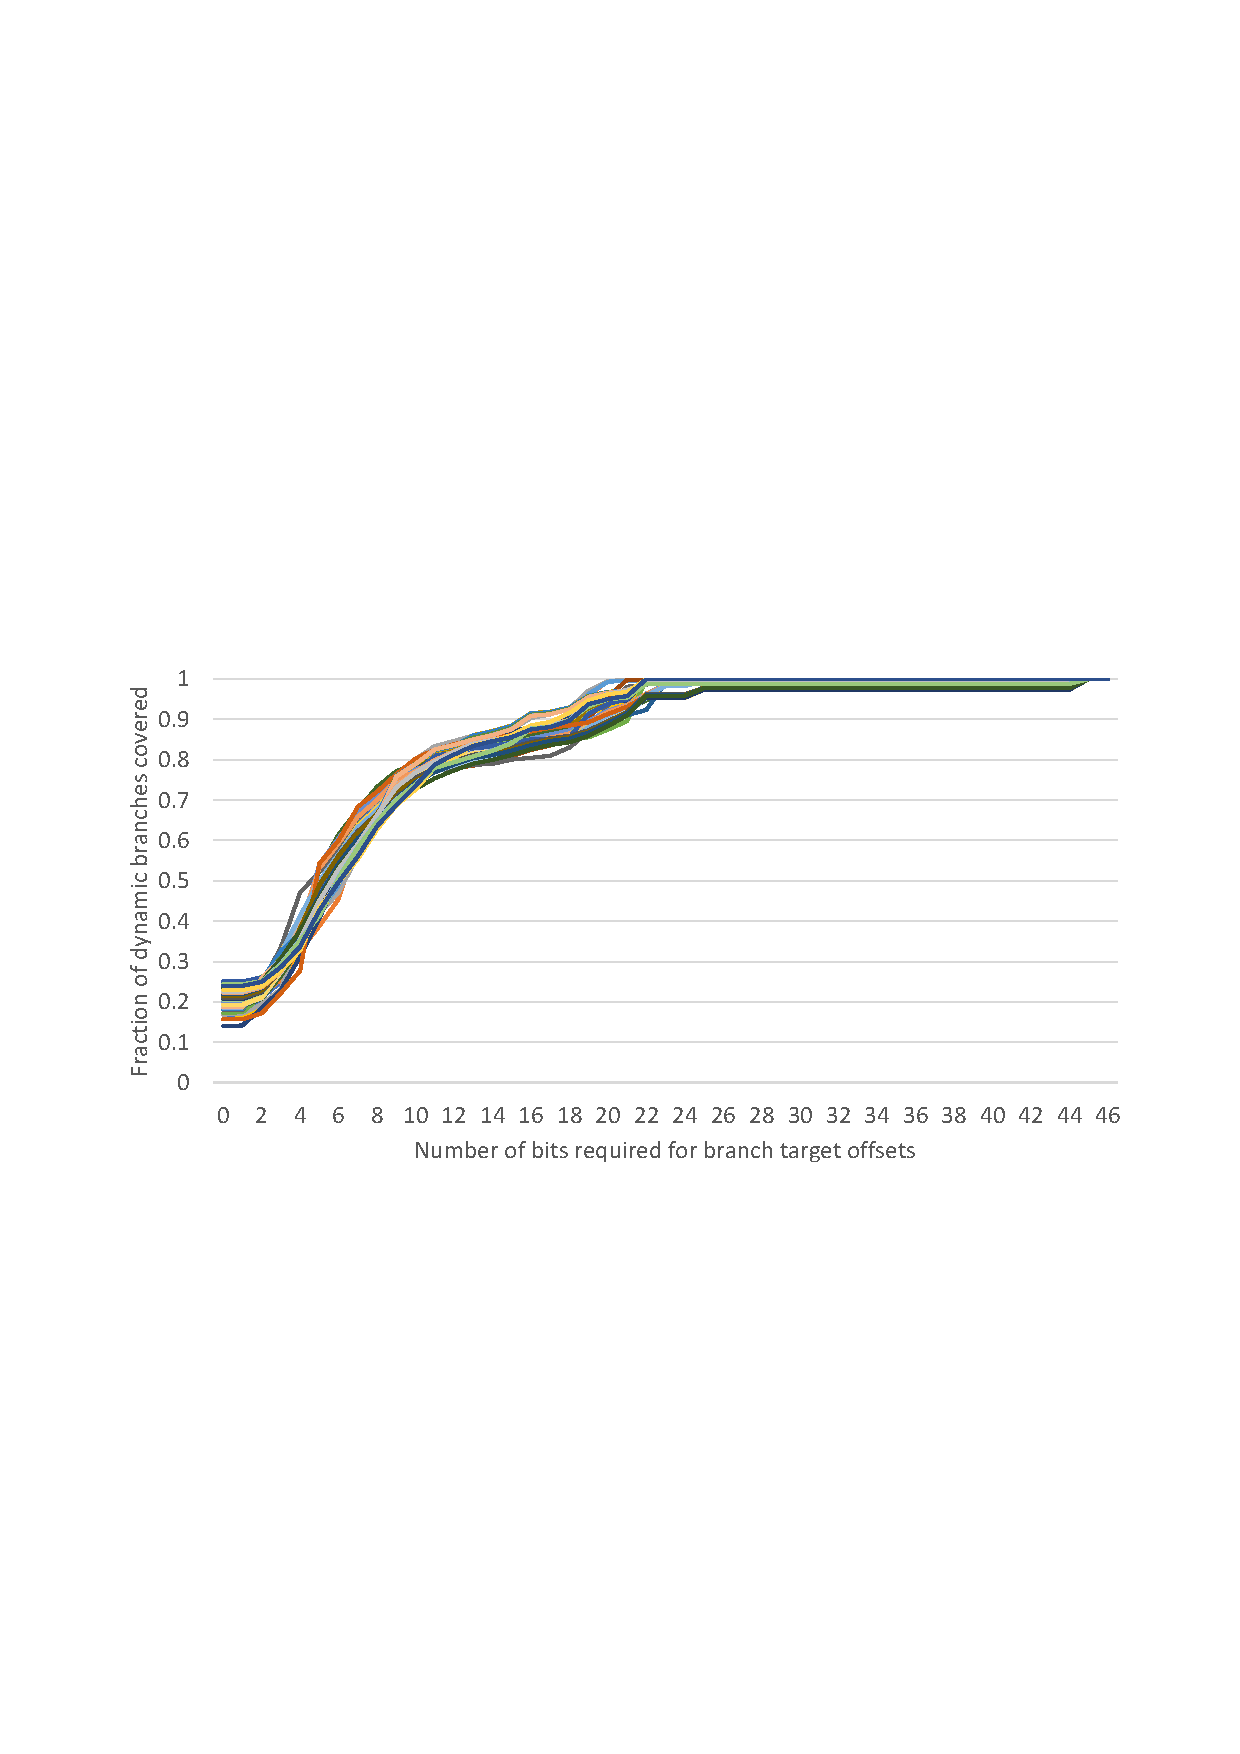
\includegraphics[width=\textwidth, trim=60 280 50 320, clip]{figures/offset_distribution.pdf}
    \caption{Distribution of branch target offsets in different workloads.}
    \label{fig:offsets}
\end{figure*}


The storage cost of branch targets accounts for a major fraction of BTB storage requirements. For example, in a conventional BTB, as depicted in \Cref{fig:conv-btb}, the target field accounts for about 72\% (46 of 64 bits) of the total BTB storage requirements. We analyze the number of bits required for branch target \emph{offsets} to assess if storing the offsets, instead of the full or compressed targets, can reduce BTB storage requirements. We define the target offset as the \textit{n} least significant bits of target address, with \textit{n} being the position of most significant bit that differs among branch PC and target. As an example, for the branch PC and target shown in \Cref{fig:concat}, the most significant bit that differs among them is at position five, whereas all bits at positions higher than five are same. Therefore, the target offset for this branch PC and target pair is `11000', i.e., the target bits from position 5 to 1. Also, as our modelled ARM v8 ISA aligns instructions at 4-byte boundaries, the two least significant bits of a target are always zeros. Therefore, we only need to store `110' as offset in the BTB.


An advantage of defining an offset as \textit{n} lower order target bits, instead of the numerical distance between branch PC and target (i.e., target - PC), is that the full target can be recovered by simply concatenating the shifted branch PC with the offset retrieved from BTB. In contrast, using numerical distance as offset would require a 48-bit adder to recover the full target from offset. 

\Cref{fig:offsets} plots the distribution of branch target offsets in the branch working sets of our workloads. The data includes both conditional and unconditional branches; hence, it comprehensively covers the full branch working set. The X-axis shows the number of bits required to store offsets, while the Y-axis plots the fraction of dynamic branches covered.

As the figure shows, short offsets dominate the distribution with 54\% of branches requiring only six bits or fewer for their offsets. A further 22\% of branches only require between 7 and 10-bits to represent their offsets. The reason why such a high fraction of offsets is short is that conditional branches dominate the dynamic branch working set, and they tend to have short offsets~\cite{boomerang}. This is because conditional branches generally guide the control flow only inside a function; meanwhile, software engineering principles favor small functions, thus restricting conditional branch target offsets to short distances. Furthermore, as discussed in \Cref{sec:background}, return instructions get their target from RAS, thus they do not need to store any target bits in BTBs. Therefore, for the purpose of this analysis, we assume 0-bit offsets for return instructions.

Perhaps surprisingly, \Cref{fig:offsets} also shows that very few branches require a large number of bits for their offset. Indeed, a meagre 1\% of branches requires more than 25 bits for their offsets. The sum of these results indicates that reserving space for the full 46-bit target address results in an appalling under-utilization of BTB storage, since 99\% of branches need at most half the number of bits needed to represent the full target address if offsets are used instead.

We gain two key insights from this analysis:

\begin{description}
\item[Key Insight 1] The targets of most branches lie relatively close in the virtual address space to the branch itself. As a result, storing the {\em distance} to the target, in the form of an offset from the branch instruction can provide drastic storage savings.

\item[Key Insight 2] The target offset sizes are unevenly distributed with 0-6 bits, 7-10 bits, and 11-25 bits required to encode the offsets of 54\%, 22\% and 23\% of branches respectively. Therefore, a single size offset field cannot provide storage optimal solution.
\end{description}
